\documentclass[12pt, openany]{report}
\usepackage[utf8]{inputenc}
\usepackage[T1]{fontenc}
\usepackage[a4paper,left=2cm,right=2cm,top=2cm,bottom=2cm]{geometry}
\usepackage[french]{babel}
\usepackage[pdftex]{graphicx}
\usepackage{enumitem}
\usepackage{array}
\usepackage{pdfpages}

\setlength{\parindent}{0cm}
\setlength{\parskip}{1ex plus 0.5ex minus 0.2ex}
\newcommand{\hsp}{\hspace{20pt}}
\newcommand{\HRule}{\rule{\linewidth}{0.5mm}}
\newcolumntype{M}[1]{>{\centering\arraybackslash}m{#1}}

\begin{document}
    \begin{titlepage}
        \begin{center}
            \textsc{\LARGE École Polytechnique de l'Université de Tours}
            \\[2cm]

            
\includegraphics{img/polytech}
            \\[2cm]

            \HRule \\[0.4cm]
            { \huge \bfseries Carnet de suivi\\[0.4cm] }

            \HRule \\[2cm]

            \begin{minipage}{0.4\textwidth}
                \begin{flushleft} \large
\textsc{Brouard} Romain\\\end{flushleft}
            \end{minipage}
            \begin{minipage}{0.4\textwidth}
                \begin{flushright} \large
\emph{Tutrice académique:}\\ Mme. \textsc{Rault} Tiffen\\
\emph{Maître d'apprentissage:}\\ M. \textsc{Berruer} Stéphane\\
\end{flushright}
            \end{minipage}

            \vfill

            {\large 1\ier{} Septembre 2023 — 31 Août 2023}


\includegraphics[width=\textwidth]{/home/romain/Bureau/Suivi/carnet-de-suivi/img/eiffage.png}


        \end{center}
    \end{titlepage}

    \setcounter{tocdepth}{1}
    \tableofcontents

    \chapter{Présentation}
\section*{Semaine 36}
\begin{tabular}{|l|l|l|l|}
\hline
Matière & Description & Evaluation & Commentaire \\ 
\hline
Remise à niveau mathématique & Cours sur les fonctions usuelles & N & com \\ 
\hline
Remise à niveau mathématique & TD sur les fonctions usuelles & N & com \\ 
\hline
Projet Accueil & Présentation du projet d'accueilQu'est ce que l'innovation?Des intervenants nous ont présentés quelques exemples d'innovations & N & com \\ 
\hline
Fresque du climat & Réalisation d'une fresque du climat avec notre groupe de projet d'accueil & N & com \\ 
\hline
Réunion de rentrée  & Réunion de rentrée POLYTECHPrésentation de la formation par apprentissage & N & com \\ 
\hline
Réunion de rentrée BDE & reubde & N & com \\ 
\hline
TOEIC & Test du TOEIC & N & com \\ 
\hline
Présentation de l'ENT & reuent & N & com \\ 
\hline
\end{tabular}

\section*{Semaine 37}
\begin{tabular}{|l|l|l|l|}
\hline
Matière & Description & Evaluation & Commentaire \\ 
\hline
Remise à niveau mathématique & remath & N & com \\ 
\hline
Anglais & math & N & com \\ 
\hline
Automatisme & autom & N & com \\ 
\hline
Remise à niveau informatique & info & N & com \\ 
\hline
Electronique & elec & N & com \\ 
\hline
Projet Accueil & proj & N & com \\ 
\hline
\end{tabular}

\section*{Semaine 38}
\begin{tabular}{|l|l|l|l|}
\hline
Matière & Description & Evaluation & Commentaire \\ 
\hline
Remise à niveau informatique & info & N & com \\ 
\hline
Anglais & andlais & N & com \\ 
\hline
Remise à niveau mathématique & maths & N & com \\ 
\hline
Automatisme & aurom & N & com \\ 
\hline
Elections délégués & dleg & N & com \\ 
\hline
Electronique & elec & N & com \\ 
\hline
\end{tabular}

\chapter{Annexes}
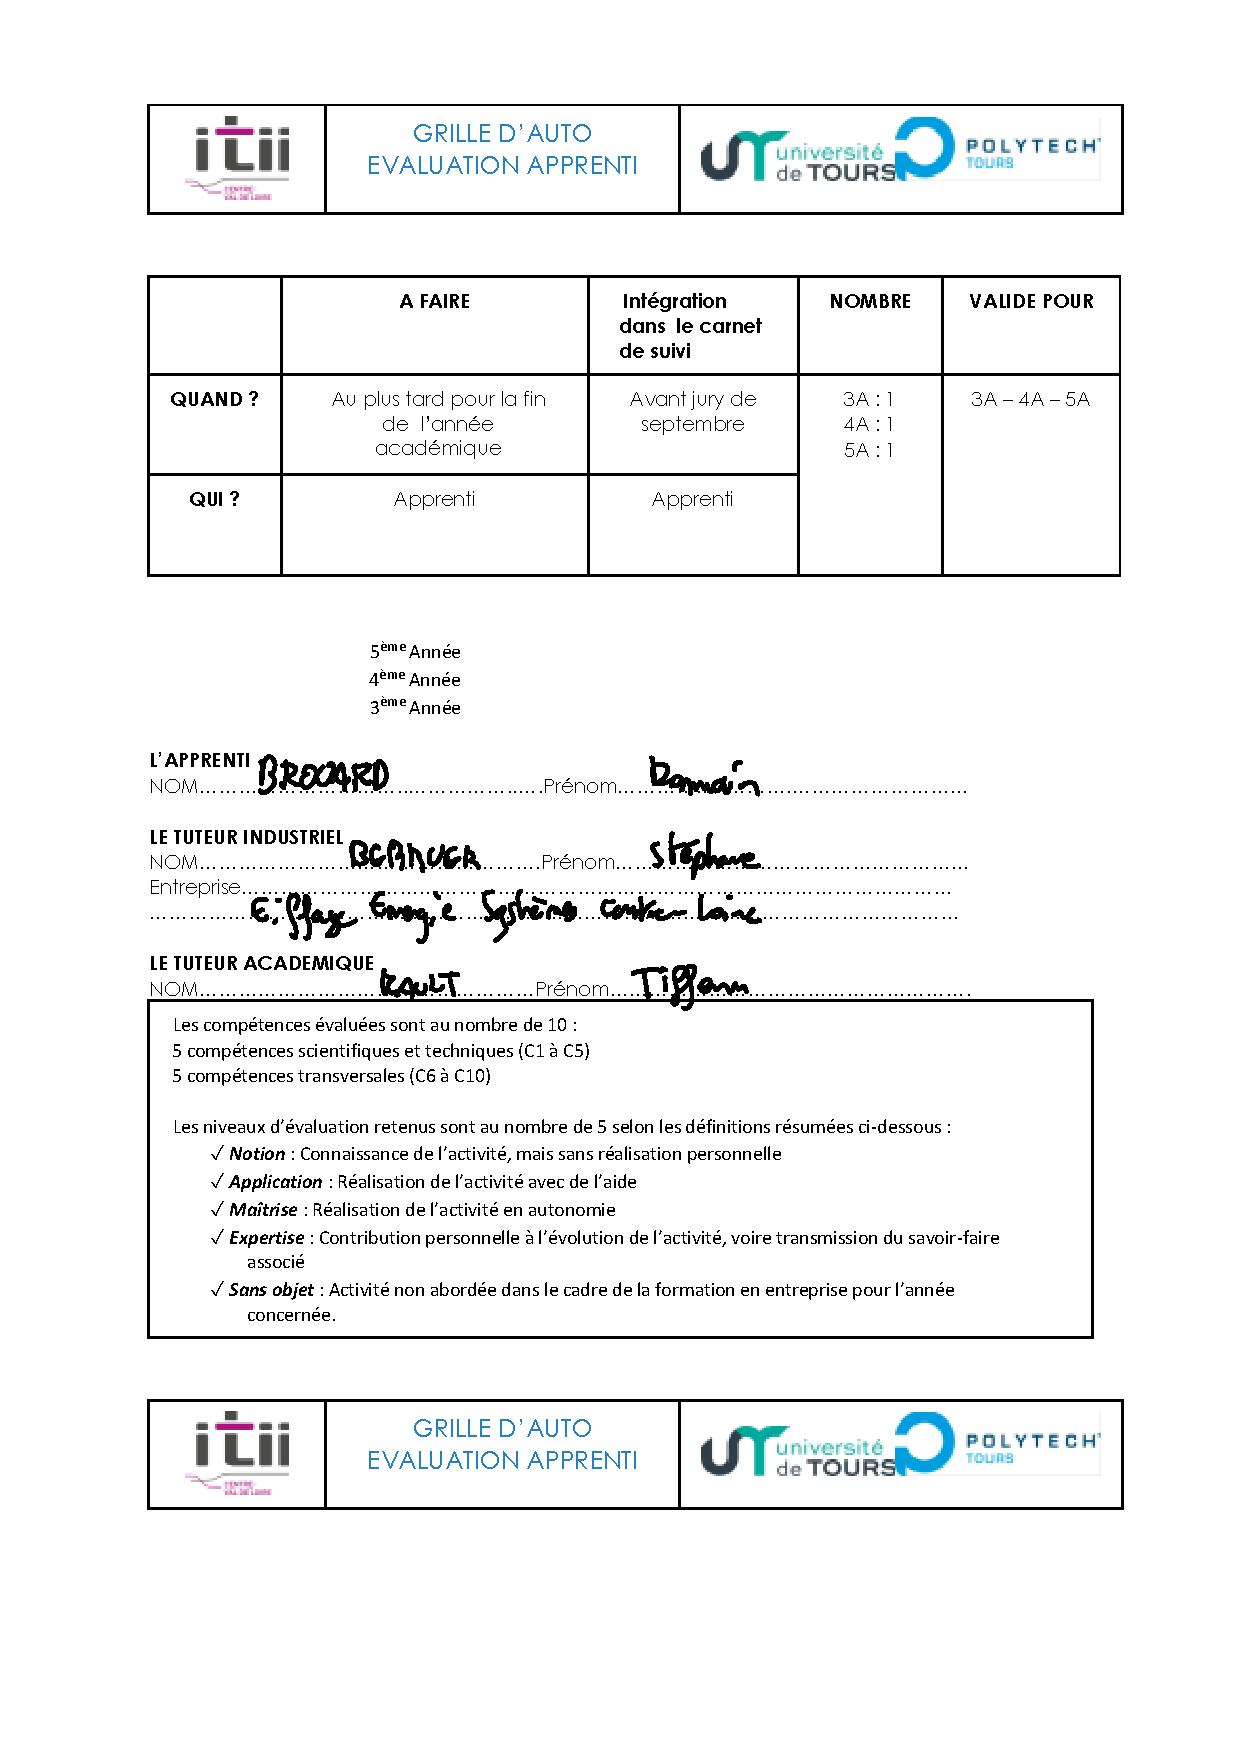
\includepdf[pages=-]{/home/romain/Bureau/Suivi/carnet-de-suivi/test/auto_eval_test.pdf}
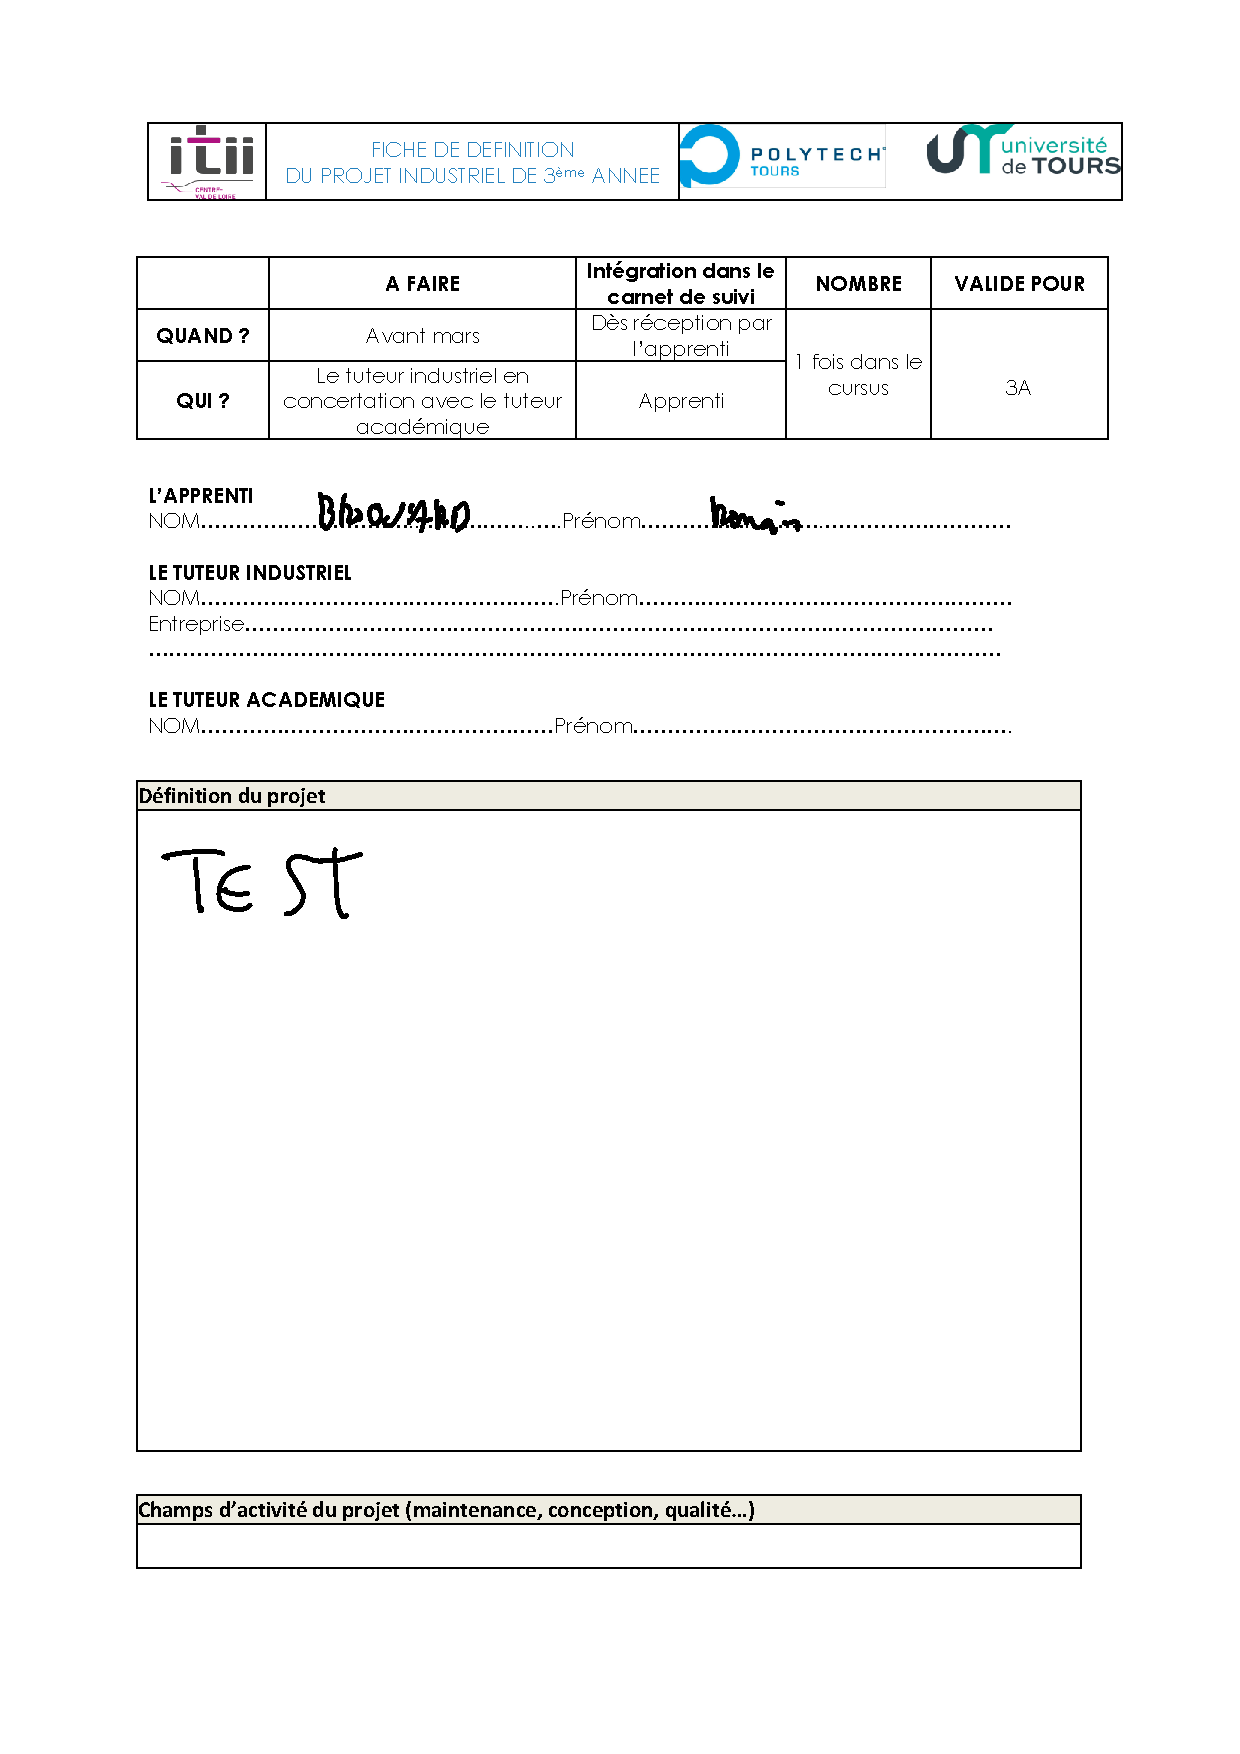
\includepdf[pages=-]{/home/romain/Bureau/Suivi/carnet-de-suivi/test/proj_indus_test.pdf}
\end{document}